\section{RTL Files and Structure}

The RTL files of the mmRISC-1 are shown in Table \ref{tb:RTLFILES}, and the RTL structure in the mmRISC-1 is shown in Figure \ref{fig:RTLSTRUCTURE}. The top layer of the mmRISC-1 (mmRISC.V) has two large domains, one is a multiple CPU (Hart) block (cpu\_top.v) and the other is a Debug block (debug\_top.v). As for the periodic interrupt timer MTIME, it is defined in the CSR but it is outside of the CPU core because it is connected to the system bus as a memory mapped peripheral. \\

Basically, the debug interface is 4-wire JTAG, but you can use 2-wire cJTAG (Compact JTAG) instead. If you use cJTAG, please add a “cJTAG to JTAG converter” (CJTAG\_2\_JTAG.v) in the same layer as the mmRISC. The conversion logic is described in the SoC chapter of this document in detail.


\begin{table}[H]
    \begin{adjustbox}{scale={1.0}{1.0}}
    \textsf{
    \begin{tabular}{|L{6cm}{3.5cm}{t}|L{10cm}{7cm}{t}|L{2cm}{2cm}{t}|}
        \hline
        %-------------------------------------
        \rowcolor{LightPurple}
        \textbf{File Name} &
        \textbf{Description} &
        \textbf{Note}
        \nextRow \hline
        %-------------------------------------
        defines\_core.v	&
        Definitions and Configurations for Core &
        ~
        \nextRow \hline
        %-------------------------------------
        defines\_chip.v &
        Definitions and Configurations for Chip	&
        ~
        \nextRow \hline
        %-------------------------------------
        mmRISC.v &
        Top Layer of mmRISC-1 &
        ~
        \nextRow \hline
        %-------------------------------------
        bus\_m\_ahb.v &
        Bridge from Internal Bus to AHB Lite &
        ~
        \nextRow \hline
        %-------------------------------------
        csr\_mtime.v &
        Memory Mapped CSR MTIME &
        ~
        \nextRow \hline
        %-------------------------------------
        cpu\_top.v &
        Top Layer of CPU (Hart) &
        ~
        \nextRow \hline
        %-------------------------------------
        cpu\_fetch.v &
        Instruction Fetch Unit &
        ~
        \nextRow \hline
        %-------------------------------------
        cpu\_pipeline.v &
        Pipeline and Decode Control &
        ~
        \nextRow \hline
        %-------------------------------------
        cpu\_datapath.v & 
        Datapath Unit &
        ~
        \nextRow \hline
        %-------------------------------------
        cpu\_csr.v &
        Machine Mode CSR &
        ~
        \nextRow \hline
        %-------------------------------------
        cpu\_csr\_int.v &
        Interrupt Controller and its CSR &
        ~
        \nextRow \hline
        %-------------------------------------
        cpu\_csr\_dbg.v &
        Debug CSR &
        ~
        \nextRow \hline
        %-------------------------------------
        cpu\_debug.v &
        Debug Support Logic &
        ~
        \nextRow \hline
        %-------------------------------------
        cpu\_fpu32.v &
        Floating Point Unit &
        ~
        \nextRow \hline
        %-------------------------------------
        debug\_top.v &
        Debugger Top &
        ~
        \nextRow \hline
        %-------------------------------------
        debug\_dtm\_jtag.v &
        Debug Transport Module with JTAG I/F &
        ~
        \nextRow \hline
        %-------------------------------------
        debug\_cdc.v &
        Clock Domain Crossing &
        ~
        \nextRow \hline
        %-------------------------------------
        debug\_dm.v &
        Debug Module &
        ~
        \nextRow \hline
        %-------------------------------------
        cjtag\_2\_jtag.v &
        Converter from cJTAG to JTAG &
        optional
        \nextRow \hline
        %-------------------------------------
    \end{tabular}
    }
    \end{adjustbox}
    \caption{RTL Files}
    \label{tb:RTLFILES}
\end{table}


\begin{figure}[H]
    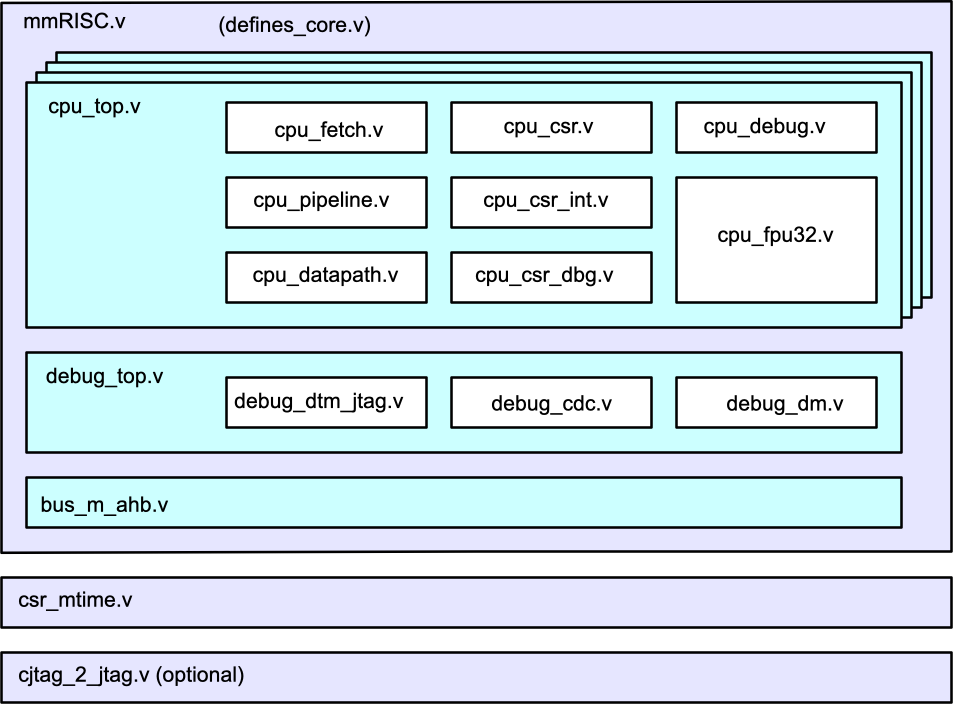
\includegraphics[width=1.0\columnwidth]{./Figure/RTLStructure.png}
    \caption{RTL Files}
    \label{fig:RTLSTRUCTURE}
\end{figure}
